\section{Resonant tuning and the absorption set}\label{sec:tuning}

\subsection{Resonant pairs and orbit closure}
By \cref{lem:modal}, the nominal flow is a linear flow on the invariant tori
$\{A_\pm=\mathrm{const}\}$ with frequency vector $(\Op,\Om)$.

\begin{definition}[Resonant pair]
A pair $(\tau,\sigma)\in\NN^2$ with $\tau>\sigma$ and $\gcd(\tau,\sigma)=1$ is
\emph{resonant} for $n$ if $\Op/\Om=\tau/\sigma$.
\end{definition}

\begin{proposition}[\citealp{juchem2026shaping}]\label{prop:resonance}
The projections of the nominal flow on $(q,\dot q)$ and $(z,\dot z)$ are closed
curves for every initial condition in $\mathcal D_0$ if and only if $\Op/\Om$ is
rational.
The pair $(\tau,\sigma)$ is resonant if and only if
\begin{equation}\label{eq:n-design}
  n=\frac{\tau-\sigma}{\sqrt{\tau\sigma}},\qquad\text{equivalently}\quad
  \Op=\frac{\tau}{\sqrt{\tau\sigma}},\ \Om=\frac{\sigma}{\sqrt{\tau\sigma}},
\end{equation}
and then every orbit is periodic with common period $P_0=2\pi\sqrt{\tau\sigma}$.
Moreover, $\dot\psi=\sigma\Op-\tau\Om=0$, so $\psi$ is a first integral of the
nominal flow, and an orbit in $\mathcal D_0$ is determined by $(A_+,A_-,\psi)$.
\end{proposition}

Throughout, $(\tau,\sigma)$ is fixed and $n$ is given by \eqref{eq:n-design}.
We also assume $\tau+\sigma\ge5$.
This excludes the low-order pairs $(2,1)$ and $(3,1)$, for which harmonics of
order up to four resonate.
It is needed in \cref{lem:averaged} and is satisfied by every practically
relevant design~\citep[cf.][Sec.~V]{juchem2026shaping}.

\subsection{The absorption set}
\citet[Thm.~1]{juchem2026shaping} showed that the \emph{impulse response}
reaches the host origin if and only if $\tau-\sigma\equiv2\pmod4$.
The following result places this criterion in the full orbit space and is the
geometric basis of the controller in \cref{sec:control}.

\begin{theorem}[Absorption set]\label{thm:absorption}
Let $(\tau,\sigma)$ be resonant, $x_0\in\mathcal D_0$, $\rho:=A_-/A_+=e^{-\eA}$
and $r:=\tau/\sigma$.
The nominal orbit through $x_0$ contains a point with $q=\dot q=0$ if and only if
\begin{enumerate}
\item[(i)] $1\le\rho\le r$, i.e.\ $-\ln(\tau/\sigma)\le\eA\le0$; and
\item[(ii)] $\psi\in\Psi^\star(\eA):=\{\sigma\vartheta_+-\tau\vartheta_- \bmod
  2\pi\}$, where $(\vartheta_+,\vartheta_-)$ ranges over the (at most four)
  solutions of $\rho\sin\vartheta_-=-\sin\vartheta_+$,
  $\rho\cos\vartheta_-=-r\cos\vartheta_+$, explicitly
  $\cos^2\vartheta_+=(\rho^2-1)/(r^2-1)$.
\end{enumerate}
In particular, for equal amplitudes ($\eA=0$),
\begin{equation}\label{eq:psi-star}
  \Psi^\star(0)=\big\{(\tau+\sigma)(2j+1)\tfrac{\pi}{2}\bmod 2\pi:\ j\in\ZZ\big\},
\end{equation}
which is a single phase if $\tau+\sigma$ is even and two phases, $\pi$ apart, if
$\tau+\sigma$ is odd.
\end{theorem}

The proof is in \cref{app:absorption}.
Geometrically, the host projection is the sum of two coaxial ellipses, with
semi-axes $(A_+,\Op A_+)$ and $(A_-,\Om A_-)$.
Their sum can vanish only if the ellipses intersect, which is condition (i).
Whether the orbit actually passes through an intersection point is then a
statement about the relative phase alone, which is condition (ii).

\begin{corollary}[Impulse response; {\citealp[Thm.~1]{juchem2026shaping}}]
\label{cor:mod4}
The impulse response ($\eA=0$, $\psi=0$) reaches the host origin if and only if
$\tau-\sigma\equiv2\pmod4$.
\end{corollary}
\begin{proof}
By \eqref{eq:psi-star}, $0\in\Psi^\star(0)$ iff $4\mid(\tau+\sigma)(2j+1)$ for
some $j$, i.e.\ iff $\tau+\sigma\equiv0\pmod4$.
For coprime $\tau,\sigma$ this holds iff both are odd and
$\tau-\sigma=(\tau+\sigma)-2\sigma\equiv2\pmod4$.
\end{proof}

\Cref{thm:absorption} changes the design interpretation of~\citet{juchem2026shaping}.
The congruence is not a property of the pair $(\tau,\sigma)$ alone; it is a
property of the relative phase that the impulse happens to produce.
Every resonant pair has absorbing orbits.
For instance, $(6,5)$, designed for containment in~\citet{juchem2026shaping}, is
absorbing at $\psi=\pm\pi/2$ (\cref{fig:tuning}(c)).
Consequently a controller that can steer $\psi$ can choose between absorption and
containment for a fixed $n$, and can thus decouple the speed requirement, which
fixes $n$ through $T_{\min}\approx\pi/n$, from the absorption requirement.
\Cref{fig:absorption} shows the absorption set for $(11,9)$.

\begin{figure}[t]
  \centering
  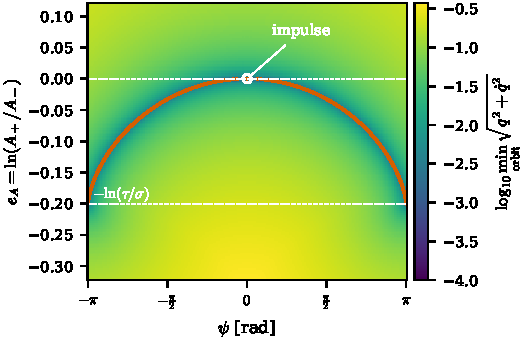
\includegraphics[width=\columnwidth]{fig_absorption.pdf}
  \caption{Minimal host radius along the resonant orbit as a function of
  $(\psi,\eA)$ for $(\tau,\sigma)=(11,9)$, $A_+=1$.
  Red: the absorption set of \cref{thm:absorption}; dashed: the band
  $-\ln(\tau/\sigma)\le\eA\le0$.
  The impulse response lies at the apex $(0,0)$.}
  \label{fig:absorption}
\end{figure}

\begin{remark}[Robustness of the absorbing target]\label{rem:apex}
At the apex $(\psi,\eA)=(0,0)$ the absorption set is tangent to $\{\eA=0\}$.
The minimal host radius therefore grows only quadratically in a phase error,
but linearly in an amplitude error with $\eA>0$ (\cref{fig:absorption}).
Interior targets $-\ln(\tau/\sigma)<\eA^\star<0$ give a transversal crossing,
with linear sensitivity in both directions.
In this paper the controller targets $(\eA,\psi)=(0,\psis)$ with
$\psis:=(\tau+\sigma)\pi/2$, consistent with~\citet{juchem2027restoring}.
\gap{Optimal absorbing target}{Quantify the minimal host energy as a function of
$(\delta\eA,\delta\psi)$ around a point of $\Psi^\star$ and choose the target
that minimises the worst case over the ISS residual set of
\cref{thm:iss-avg}. An interior target with a bias in $\eA$ may beat the apex.}
\end{remark}

\subsection{Inscribed radius and the speed--depth trade-off}
For the impulse response, $(q,\dot q)$ lies on a Lissajous curve whose convex hull
is the Minkowski sum of the ellipses above~\citep[Prop.~2]{juchem2026shaping}.
Let $r_{\mathrm{res}}$ be the radius of the largest origin-centred disc inside
the curve.
It certifies $\min_tH_q(t)=\tfrac12r_{\mathrm{res}}^2$ and vanishes exactly in
the case of \cref{cor:mod4}.
When $\tau-\sigma\not\equiv2\pmod4$, \citet[Thms.~2--4]{juchem2026shaping} locate
the minimiser near the slow-mode node $\theta\approx\pi/(\tau-\sigma)$, i.e.\
$T_{\min}\approx\pi/n$, and give an asymptotic root approximation with error
$O\big((\tau-\sigma)^2/(\tau+\sigma)^3\big)$.
\gap{Rigour of the inscribed-radius localisation}{The monotonicity argument of
\citet[Thm.~2]{juchem2026shaping} uses order-of-magnitude reasoning
($O(\cos\beta)$, ``$\approx$''). For the journal version either (a) prove it with
explicit bounds on $q\,\partial_\theta q$ versus $\dot q\,\partial_\theta\dot q$ inside the envelope-minimising
lobe, or (b) state the localisation as a numerical certificate (interval
bisection on $\dot q(\theta)=0$), which is all the design needs.}

Large $n$ (low-order pairs) gives fast but shallow exchange, and small $n$ gives
deep but slow exchange; the set $\{(r_{\mathrm{res}},T_{\min})\}$ forms a Pareto
front~\citep[Fig.~2]{juchem2026shaping}.
Requiring a pronounced beat, $(\tau+\sigma)/(\tau-\sigma)\ge10$, the fastest
absorbing impulse design is $(11,9)$, with $n=0.2010$ and $T_{\min}\approx15.6$\,s.
The next candidate with $\tau-\sigma=6$ is $(35,29)$, with $T_{\min}\approx16.7$\,s.
\citet{juchem2026shaping} reported $(41,35)$, which is not minimal; the
conclusion is unchanged.
For containment, $(6,5)$ gives $r_{\mathrm{res}}=0.0508\,v_0$.
By \cref{thm:absorption}, however, these labels refer to the \emph{impulse}
phase $\psi=0$ only.
The pair $(11,9)$ is used as the running example.

\begin{figure*}[t]
  \centering
  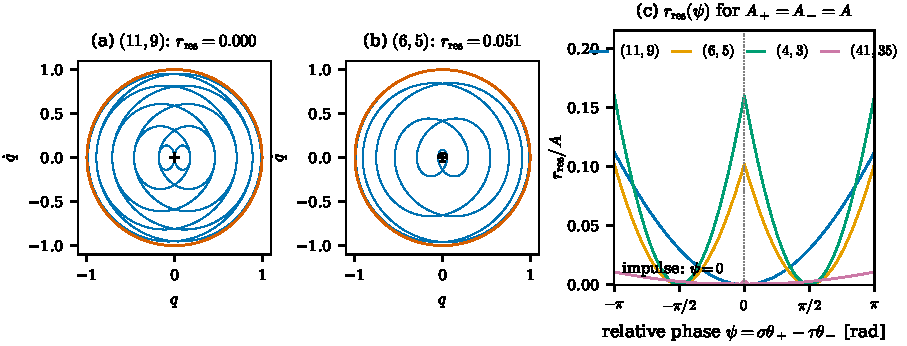
\includegraphics[width=\textwidth]{fig_tuning.pdf}
  \caption{Resonant tuning. (a)--(b) Host phase portraits of the impulse response
  ($v_0=1$) with the convex envelope (red) and the inscribed circle (dashed) for
  $(11,9)$ and $(6,5)$. (c) Inscribed radius of the orbit with $A_+=A_-$ as a
  function of the relative phase; dots mark $\Psi^\star(0)$ in
  \eqref{eq:psi-star}. Every pair is absorbing at the right phase; the
  impulse fixes $\psi=0$.}
  \label{fig:tuning}
\end{figure*}
